\documentclass[12pt,fleqn]{article}\usepackage{../common}
\begin{document}
Minimum Kapsamli Agac (Minimum Spanning Tree -MST-)

MST algorithmasi kenar agirliklarina (weights) sahip olan bir cizit (graph)
yapisi icinde minimal ve kapsayan agaci (MST) bulan algoritmaya verilen
isimdir. Mesela alttaki cizit icinde

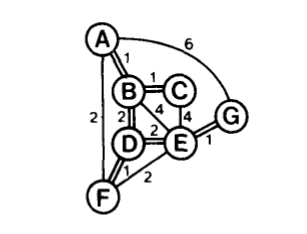
\includegraphics[height=4cm]{minspan_0.png}

MST oyle bir baglanti yapisidir ki bastan sona, herhangi bir noktadan
(node) bir digerine gecis yapilabilsin, ve bu tum yollarin toplami en
minimal olsun. Dikkat, herhangi bir noktadan digerine giden yol en az olsun
demiyoruz, bu durumda problem en kisa yol (shortest path) problemi
olurdu, ki bu problemi {\em Dinamik Programlama} yazisinda gorduk. Burada
gorecegimiz kapsayan agacin {\em toplaminin} minimal olmasidir. 

Kapsayan agac (spanning tree) kavramini tanimlamak gerekirse, bir cizitin
kapsayan agaci orijinal cizitin tum noktalarina sahip olmalidir, agac
icinde hicbir dongu (cycle) olmamalidir. Dongu derken bir noktadan digerine
atlaya atlaya giderken bizi donup tekrar ayni yere getirebilecek turden
``kapali devre'' tur bir donguden bahsediyoruz - bu mumkun
olmamalidir. Ayrica cizit baglantili olmalidir, yani bir kismi diger
kismindan kopuk bir cizit uzerinde MST bulunamaz. 

Minimum kapsayici agac ise bu tur pek cok alternatif agaclarin icinde en az
agirlikli olanidir. Not, bir cizitin MST cozumu tekil (unique) olmayabilir,
ayni agirlikta birden fazla degisik agac mumkundur. Mesela ustteki cizit
icin mumkun MST'ler altta goruluyor,

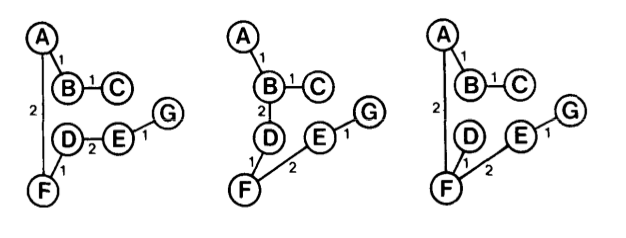
\includegraphics[height=4cm]{minspan_1.png}

Kontrol edilebilir, ustteki her agacin kenar toplami 8'dir. Bu agaclarin
her biri bir MST olarak kabul edilebilir.

Uygulama baglaminda MST bulma algoritmasinin ne kadar kullanisli olacagi
goruluyor herhalde; mesela elektrik hatlari, telefon iletisim hatlari
tasarlarken MST kullanilabilir, toplam baglantisi en az olan bir ag yapisi
her iki durumda da kullanisli olur. Biyolojik, kimyasal aglarin analizinde
bile MST kullanilmaktadir.

Agaclarin Ozellikleri (Properties of Trees)

Baslamadan once bir agaci agac yapan iki onemli ozelligini belirtelim

1) Elde olan, tanim itibariyle agac olan bir agacin arasinda baglanti
olmayan iki noktasini birlestiren bir kenar koyarsak bu agacta bir dongu
yaratmis oluruz.

2) Elde olan bir agacin herhangi bir kenarini cikartirsak bu agaci
``kopartmis'' oluruz, birbiriyle baglantisiz iki alt-agac ortaya cikar.

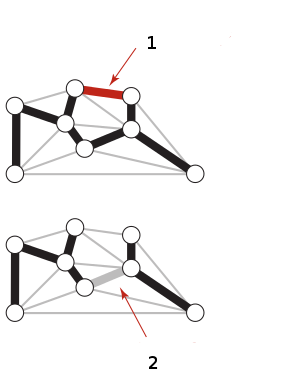
\includegraphics[height=8cm]{graph_prop.png}

Resimde her iki durumu goruyoruz. Bu iki ozellik cok onemli, cunku onlari
MST'lerin cok temel bir ozelligini ispatlamak icin kullanacagiz.

Tanim

Kesik (cut): Bir cizit uzerindeki kesik, bir ciziti birbiriyle alakasiz,
baglantisiz iki parcaya / kumeye boler. 

Not: Dikkat bir kesik birden fazla kenari kapsayabilir, cunku bir ciziti
kesmekten bahsediyoruz. Bir agactan bahsediyor olsaydik, yukarida
belirttigimiz gibi, tek bir kenari kesmek yeterli olurdu.

Birlestiren kenar (crossing edge): birbirinden baglantisiz iki kumedeki
herhangi bir noktayi diger kumedeki herhangi bir diger noktayla birlestiren
bir kenardir.

Onerme (Proposition)

Herhangi bir ciziti alalim, ve bu cizitteki bir kesik icindeki (yani
kopardigi tum kenarlar) icindeki minimum birlestiren kenar o cizitin MST'sinin
icinde olmalidir. 

Ispat

Bu ispat tersini yanlislama (proof by contradiction) yontemini
kullanacak. Diyelim ki bir kesik var, ve o kesikteki $e$ minimum
birlestiren kenar. Bu cizitin MST'si $T$ olsun. Simdi $e$'nin $T$'nin
icinde olmadigi durumu dusunelim (yani onermenin dediginin tersi), ve
diyelim ki simdi $e$'yi alip $T$'ye ekliyoruz. Yeni bir cizit ortaya
cikardi, fakat daha once dedigimiz gibi, $T$'ye bir kenar eklemek ona ayni
zamanda bir dongu eklemek demektir, ki bu dongunun icinde en az bir diger
kenar $f$ olacaktir (cunku $e$ MST'de olmadigina gore orada baska bir sey
var), ki bu $f$, $e$'den buyuktur. Fakat o zaman $f$'yi kesip onun yerine
daha az agirlikta olan $e$'yi ekleyince MST'yi, hem de daha az agirlikla
elde etmis olmaz miydik? Evet. Demek ki $e$'nin MST icinde olmamasi
imkansizdir cunku MST tanim itibariyle en minimal agirliga sahip olmalidir.

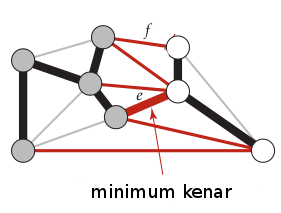
\includegraphics[height=5cm]{cross_edge.png}


\begin{minted}[fontsize=\footnotesize]{python}
G1 = {
  'a': {'b':1, 'f':2, 'g': 6},
  'b': {'a':1, 'c':1},
  'c': {'b':1},
  'd': {'f':1, 'e':2},
  'e': {'d':2, 'g':1},
  'f': {'a':2, 'd':1},
  'g': {'e':1, 'a': 6}
}
\end{minted}


\begin{minted}[fontsize=\footnotesize]{python}
def find(C, u):
    if C[u] != u:
        C[u] = find(C, C[u])                    # Path compression
    return C[u]

def union(C, R, u, v):
    u, v = find(C, u), find(C, v)
    if R[u] > R[v]:                             # Union by rank
        C[v] = u
    else:
        C[u] = v
    if R[u] == R[v]:                            # A tie: Move v up a level
        R[v] += 1

def kruskal(G):
    E = [(G[u][v],u,v) for u in G for v in G[u]]
    T = set()
    C, R = {u:u for u in G}, {u:0 for u in G}   # Comp. reps and ranks
    print list(sorted(E))
    for _, u, v in sorted(E):
        if find(C, u) != find(C, v):
            T.add((u, v))
            print (u, v)
            union(C, R, u, v)
    return T

print list(kruskal(G1))
\end{minted}

\begin{verbatim}
[(1, 'a', 'b'), (1, 'b', 'a'), (1, 'b', 'c'), (1, 'c', 'b'), (1, 'd', 'f'),
(1, 'e', 'g'), (1, 'f', 'd'), (1, 'g', 'e'), (2, 'a', 'f'), (2, 'd', 'e'),
(2, 'e', 'd'), (2, 'f', 'a'), (6, 'a', 'g'), (6, 'g', 'a')] 
('a', 'b')
('b', 'c')
('d', 'f')
('e', 'g')
('a', 'f')
('d', 'e')
[('d', 'e'), ('e', 'g'), ('d', 'f'), ('b', 'c'), ('a', 'f'), ('a', 'b')]
\end{verbatim}

\begin{minted}[fontsize=\footnotesize]{python}
m = 100 * 1000
print m**2
print np.log(m)
print m*np.log(m)
\end{minted}

\begin{verbatim}
10000000000
11.512925465
1151292.5465
\end{verbatim}


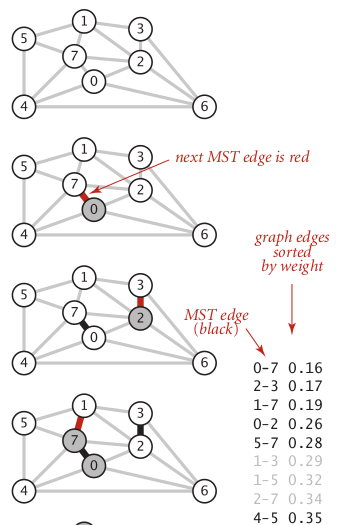
\includegraphics[height=9cm]{sedge_krus_1.png}

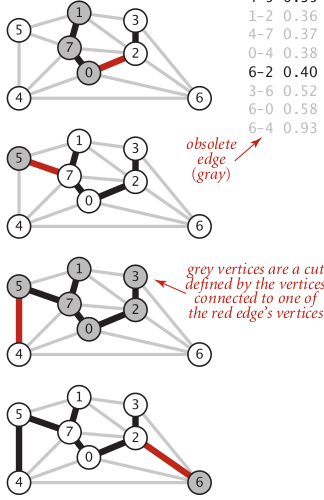
\includegraphics[height=9cm]{sedge_krus_2.png}


\begin{minted}[fontsize=\footnotesize]{python}
G2 = {
  0: {7: 0.16, 4: 0.38, 2: 0.26, 6: 0.58},
  1: {5: 0.32, 2: 0.36, 3: 0.29, 7: 0.19},
  2: {0: 0.26, 1: 0.36, 3: 0.17, 6: 0.40, 7: 0.34},
  3: {1: 0.29, 2: 0.17, 6: 0.52},
  4: {0: 0.38, 5: 0.35, 7: 0.37, 6: 0.93},
  5: {1: 0.32, 4: 0.35, 7: 0.28},
  6: {0: 0.58, 2: 0.40, 3: 0.52, 4: 0.93},
  7: {0: 0.16, 1: 0.19, 5: 0.28, 4: 0.37, 2: 0.34, 1: 0.19}
} 

print list(kruskal(G2))
\end{minted}

\begin{verbatim}
[(0.16, 0, 7), (0.16, 7, 0), (0.17, 2, 3), (0.17, 3, 2), (0.19, 1, 7),
(0.19, 7, 1), (0.26, 0, 2), (0.26, 2, 0), (0.28, 5, 7), (0.28, 7, 5),
(0.29, 1, 3), (0.29, 3, 1), (0.32, 1, 5), (0.32, 5, 1), (0.34, 2, 7),
(0.34, 7, 2), (0.35, 4, 5), (0.35, 5, 4), (0.36, 1, 2), (0.36, 2, 1),
(0.37, 4, 7), (0.37, 7, 4), (0.38, 0, 4), (0.38, 4, 0), (0.4, 2, 6), (0.4,
6, 2), (0.52, 3, 6), (0.52, 6, 3), (0.58, 0, 6), (0.58, 6, 0), (0.93, 4,
6), (0.93, 6, 4)] 
(0, 7)
(2, 3)
(1, 7)
(0, 2)
(5, 7)
(4, 5)
(2, 6)
[(2, 6), (4, 5), (5, 7), (0, 7), (2, 3), (1, 7), (0, 2)]
\end{verbatim}


















Sedgewick, R. {\em Algorithms}, sf. 409

Sedgewick, R. {\em Algorithms, 4rd Edition}, sf. 624

Heatland, {\em Python Algorithms}

\end{document}
